\documentclass[12pt]{article}


\usepackage[utf8]{inputenc}
\usepackage[spanish]{babel}
\usepackage[margin = 2.54cm]{geometry}
\usepackage{graphicx}
\usepackage{bm}
\usepackage{amsmath}
\usepackage{xcolor}
\usepackage{enumitem}
\usepackage{gensymb}


% ----------------- UTILIDADES PARA DAR UN MEJOR FORMATO DE DOCUMENTO -----------------  


\definecolor{azul}{rgb}{0.0039, 0.3098, 0.6196}


% Formato para el indice general ...........
\makeatletter
    \renewcommand{\@dotsep}{1.5}
    \renewcommand{\l@section}{\@dottedtocline{1}{1.5em}{2.3em}}
    \renewcommand{\l@subsection}{\@dottedtocline{2}{3.8em}{3.2em}}
    \renewcommand{\l@subsubsection}{\@dottedtocline{3}{7.0em}{4.1em}}
\makeatother

% --------- COMANDOS PERSONALIZADOS PARA LA PORTADA DE LAS TAREAS, TRABAJOS Y PROYECTOS ---------

\newcommand{\rutaLogo}[1]{\newcommand{\RutaLogo}{#1}}
\newcommand{\tema}[1]{\newcommand{\Tema}{#1}}
\newcommand{\etiquetaAutores}[1]{\newcommand{\EtiquetaAutores}{#1}}
\newcommand{\alumno}[1]{\newcommand{\Alumno}{#1}}
\newcommand{\materia}[1]{\newcommand{\Materia}{#1}}
\newcommand{\docente}[1]{\newcommand{\Docente}{#1}}
\newcommand{\ciclo}[1]{\newcommand{\Ciclo}{#1}}
\newcommand{\fecha}[1]{\newcommand{\Fecha}{#1}}
\newcommand{\periodo}[1]{\newcommand{\Periodo}{#1}}



\rutaLogo{../../../docs/img/logo-ista.png}
\tema{\\ \vspace{0.8cm} Tarea de lección de la unidad N\degree1 \\ \vspace{1.5cm}}
\etiquetaAutores{Integrantes: }
\alumno{Juan Orellana\\ Freddy Moltalván\\ Adrian Sumba\\ Eduardo Mendieta \vspace{0.8cm}}
\materia{Probabilidad y estadística \vspace{0.8cm}}
\docente{Eco. Hermann Seminario \vspace{0.8cm}}
\ciclo{Segundo ciclo \vspace{0.8cm}}
\fecha{25/11/2024 \vspace{0.8cm}}
\periodo{ 2024 - II}


\begin{document}
    \begin{titlepage}

    \centering

    \includegraphics[width=0.11\textwidth]{\RutaLogo} 

    \vspace{0.3cm}
    \textcolor{azul}{\Large \textbf{Instituto Superior Universitario Tecnológico del Azuay \\}}
    \vspace{0.3cm}
    \textcolor{azul}{\Large \textbf{Tecnología Superior en Big Data}}
    
    % 1. ---------------- TEMA -------------------------
    
    {\Large\textbf{\Tema}}
    
    % 2. ---------------- AUTOR(ES) -------------------------
    \textcolor{azul}{\large \textbf{\EtiquetaAutores} \\}
    \vspace{0.3cm}
    {\large \Alumno}

    % 3. ---------------- MATERIA -------------------------
    \textcolor{azul}{\large \textbf{Materia:} \\}
    \vspace{0.3cm}
    {\large \Materia}


    % 3. ---------------- DOCENTE -------------------------
    \textcolor{azul}{\large \textbf{Docente:} \\}
    \vspace{0.3cm}
    {\large \Docente}


    % 3. ---------------- Ciclo -------------------------
    \textcolor{azul}{\large \textbf{Ciclo:} \\}
    \vspace{0.3cm}
    {\large \Ciclo}


    % 3. ---------------- FECHA -------------------------
    \textcolor{azul}{\large \textbf{Fecha:} \\}
    \vspace{0.3cm}
    {\large \Fecha}

    % 3. ---------------- PERIODO -------------------------
    \textcolor{azul}{\large \textbf{Periodo Académico:} \\}
    \vspace{0.3cm}
    {\large \Periodo}
 
\end{titlepage}


    \section*{\centering  Tarea de lección de la unidad N\degree1} 
    \vspace{0.5cm}\textbf{En base a los siguientes ejercicios de tablas de contingencia, elabore las
    probabilidades: marginal, conjunta y condicional, además interprete los
    resultados y genere las conclusiones:} \vspace{0.5cm}

    \section*{\centering Tabla de contingencia y cálculo de probabilidades}

        \vspace{0.5cm}\textbf{Se evalúa si existe relación entre el género del usuario y el tipo de
        contenido preferido (películas o series) en una plataforma de
        streaming.} \vspace{0.5cm}

        \begin{figure}[ht]
            \centering
            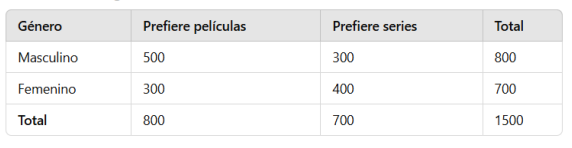
\includegraphics[width=1\textwidth]{img/tabla_contigencia.png}
        \end{figure}

        \begin{enumerate}
            \item \textbf{Probabilidad conjunta:}
                \begin{enumerate}
                    \item $A = $ Masculino y prefiere peliculas, $N =$ total:
                        \[P = \frac{A}{N} = \frac{500}{1500} = 0.3333 = 33.33\%\]
                    \item $A = $ Masculino y prefiere series, $N =$ total:
                        \[P = \frac{A}{N} = \frac{300}{1500} = 0.2 = 20\%\]
                    \item $A = $ Femenino y prefiere peliculas, $N =$ total:
                        \[P = \frac{A}{N} = \frac{300}{1500} = 0.2 = 20\%\]
                    \item $A = $ Femenino y prefiere series, $N =$ total:
                        \[P = \frac{A}{N} = \frac{400}{1500} = 0.2667 = 26.67\%\]
                \end{enumerate}

                \texttt{Conclusión:} Las películas son más apreciadas por los hombres (33,33\%), en cambio, las series 
                tienen una inclinación ligeramente superior entre las mujeres (26,67\%). 
                Las películas (800 personas) superan a las series (700), aunque las preferencias fluctúan dependiendo del género, 
                siendo la mezcla menos habitual la de hombres que prefieren las series (20\%). 

            \item \textbf{Probabilidad marginal:}
                \begin{enumerate}
                    \item $A = $Probabilidad de que les gusta las series, $N =$ total:
                        \[P = \frac{A}{N} = \frac{700}{1500} = 0.46 = 46\%\]
                    \item $A = $Probabilidad de que les gusta las peliculas, $N =$ total:
                        \[P = \frac{A}{N} = \frac{800}{1500} = 0.53 = 53\%\]
                    \item $A = $Probabilidad de que sea masculino, $N =$ total:
                        \[P = \frac{A}{N} = \frac{800}{1500} = 0.53 = 53\%\]
                    \item $A = $Probabilidad de que sea femenino, $N =$ total:
                        \[P = \frac{A}{N} = \frac{700}{1500} = 0.46 = 46\%\]
                \end{enumerate}

                \texttt{Conclusiones:} 
                \begin{itemize}
                    \item La probabilidad total del publico femenino es equivalente al total de las series con un 46\%.
                    \item La probabilidad total del publico masculino es equivalente al total de la probabilidad de las peliculas con un total del 53\%.
                \end{itemize}

            \item \textbf{Probabilidad condicional:}
                \begin{enumerate}
                    \item $A = $Probabilidad de que le guste las peliculas, $B = $dado que sea femenino:
                        \[P(A \cap B) = \frac{A \cap B}{P(B)} = \frac{300}{700} = 0.42 = 42\%\]
                    \item $A = $Probabilidad de que le guste las peliculas, $B = $dado que sea Masculino:
                        \[P(A \cap B) = \frac{A \cap B}{P(B)} = \frac{500}{800} = 0.625 = 62.5\%\]
                    \item $A = $Probabilidad de que le guste las series, $B = $ dado que sea femenino:
                        \[P(A \cap B) = \frac{A \cap B}{P(B)} = \frac{400}{700} = 0.57 = 57 \%\]
                    \item $A = $Probabilidad de que le guste las series, $B = $dado que sea Masculino: 
                        \[P(A \cap B) = \frac{A \cap B}{P(B)} = \frac{300}{800} = 0.375 = 37.5\%\]
                \end{enumerate}
                \texttt{Conclusiones:} 
                \begin{itemize}
                    \item Los resultados muestran que los usuarios de la plataforma tienen diferentes preferencias según su género, prefiriendo las mujeres series y los hombres películas.
                    \item Si la plataforma quiere atraer a más público femenino, podría considerar agregar más contenido de series. Por otro lado, si quiere atraer a más espectadores masculinos, puedes reforzar el catálogo de películas.
                    \item Es mas probable que un espectador que ve una pelicula sea del genero masculino, que uno que vea una serie y sea del genero femenino.
                \end{itemize}
                
        \end{enumerate}

\end{document}